% DEC-066 results and discussion draft (paper-first).  Insert into a manuscript with \usepackage{graphicx,booktabs,amsmath}.  Tables: IEEE39_DEC066_tables.tex (generated from CSV).
% Every number cites a table, figure or data file (IEEE39_DEC066_*.csv in artifacts/).  Items marked \todo{} are pending evidence or review.  RMS/phasor simulation (ANDES), not EMT.
\providecommand{\todo}[1]{\textbf{[PENDING: #1]}}

\section{Results and Discussion}
\label{sec:results}

\subsection{Experimental setup}
\label{sec:setup}
The study uses the IEEE 39-bus network with six synchronous generators (SG) and four grid-forming (GFM) resources, ten monitored units, simulated with ANDES 2.0.0 (implicit trapezoidal rule, $\Delta t=2^{-8}$~s with local refinement $\Delta t/16$ on $[t_e-\Delta t,t_e+0.5]$~s, tolerance $10^{-4}$, event at $t_e=5$~s, 200~s horizon). The preventive design acts on 19 variables: the active-power set-points of nine units and ten voltage set-points; SG39 is the balancing (slack) unit. The disturbances are active-power load steps of 0.293, 0.586 and 0.878~pu (29.3, 58.6, 87.8~MW on the 100~MVA base; severities S1, S2, S3). Two operating conditions are used: OC1 (100\,\% load) and OC2 (90\,\% load). The blind evaluation cells are the buses 21, 31 and 39 with the three severities, for each dispatch (36 runs with the secondary controller B5$'$, plus 18 comparison runs with other controllers). These 54 runs are historical results obtained under a TEST access rule that was modified after the tuning stage; they are used here as retrospective evidence and not as a pre-registered blind test.

\emph{Metrics.} The limit studied is the operating Pmax of each unit in the case data, applied to the delivered active power; it is not claimed to be a physical instantaneous protection. The margin is $m=\min_i(\mathrm{Pmax}_i-P_i(t))$ over a stated window. A cell is SAFE if the 0--50~ms margin is $\ge U_{D8}=0.0109$~pu, UNSAFE if $\le-U_{D8}$ and NUMERICALLY INDETERMINATE otherwise; after 50~ms, and for $Q$, $S$ and voltage, the check is binary (rule M3V-1). $U_{D8}$ is an empirical numerical band from a local refinement study, not a mathematical bound. Dispatches are compared by $\sum|\Delta P|$ over the nine decision units against the M0 dispatch of the same group and, where recorded, against the original case dispatch; $J$ is a normalised displacement and sharing cost, not an economic cost (Table~\ref{tab:dispatches}).

% Generated by dec066_paper_latex_tables.py from IEEE39_DEC066_T*.csv (DEC-066). Do not edit by hand.
\begin{table*}[t]
\centering\footnotesize
\caption{Preventive dispatches used in this study. $J$ is a normalised displacement/pattern cost, not an economic cost. $\sum|\Delta P|$ is over the nine decision units (slack excluded), in MW on the 100~MVA base, against the M0 dispatch of the same group and, where recorded, against the original case dispatch. Min.\ margin is the smallest predicted design margin as recorded in the state file. Group A: DEC-054 design set; group B: DEC-055/059--061 design sets (OC1 and OC2). All optimisations are SLSQP runs with predictor-based constraints; none is certified optimal.}
\label{tab:dispatches}
\resizebox{\linewidth}{!}{\begin{tabular}{llllrrrrrr}
\toprule
OC & Method & Status & $J$ & $\sum|\Delta P|$ vs M0 & vs case & Min.\ margin & KKT & Time (s) & Plant eval.\\
\midrule
OC1-eq & M0 & feas.\ pred. & 1.261 & 0.0 & 4.2 & -0.1548 & 0.065 & 146 & --\\
OC1-eq & M1 (rho=0.070) & feas.\ pred. & 3.321 & 156.1 & 153.0 & 0.0285 & -- & -- & --\\
OC1-eq & M2 & feas.\ pred. & 1.299 & 15.7 & 16.7 & -0.1546 & 0.068 & 1279 & 523\\
OC1-eq & M3 & feas.\ pred. & 1.478 & 44.2 & 43.3 & -0.0000 & 0.070 & 1452 & 376\\
OC1 & M0 & local opt. & 1.261 & 0.0 & -- & -- & 0.002 & 276 & --\\
OC1 & M3 & feas.\ pred. & 1.681 & 55.3 & -- & -- & 0.062 & 1489 & 440\\
OC1 & M3+OS & feas.\ pred. & 1.759 & 62.1 & 61.2 & -- & 0.058 & 664 & 394\\
OC1 & M3+OS cut & feas.\ pred. & 1.876 & 77.9 & 76.8 & -- & 0.617 & 1354 & 792\\
OC1 & M3+OS rev3 & feas.\ pred. & 2.399 & 101.1 & 99.4 & -0.0096 & 3.390 & 641 & 435\\
OC2 & M0 & feas.\ pred. & 2.127 & 0.0 & -- & -- & 0.010 & 254 & --\\
OC2 & M3 & feas.\ pred. & 2.127 & 0.1 & -- & -- & 0.065 & 1606 & 483\\
OC2 & M3+OS & feas.\ pred. & 2.127 & 0.1 & 5.5 & -- & 0.065 & 728 & 483\\
\bottomrule
\end{tabular}}
\end{table*}

\begin{table*}[t]
\centering\footnotesize
\caption{Observed safety of the 36 blind cells (ANDES time-domain, 0--195~s after the event, B5$'$ controller). Class by the frozen rule M3V-1: delivered-power margin to Pmax within the first 50~ms with the numerical band $U_{D8}=0.0109$~pu; binary after 50~ms and for Q, S and voltage. Worst margin: smallest Pmax margin over 0--195~s. Counts are listed as S1/S2/S3 (three cells per severity). Peak window: where the worst margin occurs (J: first stored sample, F: 0--50~ms, M: 50~ms--10~s, S: 10--195~s). QSV: cells with an observed Q, S or voltage-band violation.}
\label{tab:observed}
\resizebox{\linewidth}{!}{\begin{tabular}{lcccccrcc}
\toprule
OC / dispatch & SAFE (S1/S2/S3) & INDET. & UNSAFE (S1/S2/S3) & False SAFE (50~ms) & Inadm.\ at jump & Worst margin & Peak J/F/M/S & QSV\\
\midrule
OC1 M0 & 1/0/0 & 1 & 1/3/3 & 2 & 5 & -0.444 & 0/5/4/0 & 1\\
OC1 M3+OS rev3 & 3/2/2 & 0 & 0/1/1 & 0 & 2 & -0.258 & 0/4/0/5 & 0\\
OC2 M0 & 3/3/3 & 0 & 0/0/0 & 0 & 0 & 0.209 & 0/4/5/0 & 0\\
OC2 M3+OS & 3/3/3 & 0 & 0/0/0 & 0 & 0 & 0.209 & 0/4/5/0 & 0\\
\bottomrule
\end{tabular}}
\end{table*}

\begin{table*}[t]
\centering\footnotesize
\caption{Accuracy of the predicted worst Pmax margin against the stored time-domain series. $e=$ observed $-$ predicted margin (positive: conservative prediction). 50~ms: dense predictor, observed over $[t_e,t_e+50~\mathrm{ms}]$; 195~s: M3 grid predictor, observed over $[t_e,195~\mathrm{s}]$. The 195~s RMSE excluding divergent predictions (margin magnitude $\ge1$~pu) is also given. Class counts are against the observed class over 0--195~s.}
\label{tab:predictor}
\resizebox{\linewidth}{!}{\begin{tabular}{lrrrrrrrrr}
\toprule
Group & $n$ & Bias$_{50}$ & RMSE$_{50}$ & RMSE$_{195}$ & RMSE$_{195}^{\rm excl}$ & FS$_{50}$ & FU$_{50}$ & FS$_{195}$ & FU$_{195}$\\
\midrule
OC1 M0 & 9 & 0.00007 & 0.00012 & 3.845 & 0.1586 & 2 & 0 & 0 & 1\\
OC1 rev3 & 9 & 0.00008 & 0.00012 & 0.039 & 0.0388 & 0 & 0 & 0 & 0\\
OC2 M0 & 9 & 0.00027 & 0.00062 & 0.011 & 0.0106 & 0 & 0 & 0 & 0\\
OC2 M3+OS & 9 & 0.00027 & 0.00062 & 0.011 & 0.0106 & 0 & 0 & 0 & 0\\
ALL 36 & 36 & 0.00017 & 0.00045 & 1.923 & 0.0787 & 2 & 0 & 0 & 1\\
\bottomrule
\multicolumn{10}{l}{FS: false SAFE (predicted SAFE, observed not SAFE); FU: false UNSAFE. Margins in pu.}\\
\end{tabular}}
\end{table*}

\begin{table}[t]
\centering\footnotesize
\caption{Retrospective horizon sweep of the predicted classification (predicted margin over $[t_e,t_e+T_c]$ on the saved M3 grid, no parabolic refinement). Exploratory: the horizon was examined on the same 36 observed cells and it is not a blind result.}
\label{tab:horizon}
\resizebox{\linewidth}{!}{\begin{tabular}{lrrrrr}
\toprule
Group & $T_c$ (s) & Agree & False SAFE & False UNSAFE & Pred.\ INDET.\\
\midrule
ALL & 0.05 & 34/36 & 2 & 0 & 1\\
ALL & 1.00 & 35/36 & 0 & 0 & 2\\
ALL & 10.00 & 35/36 & 0 & 0 & 2\\
ALL & 60.00 & 35/36 & 0 & 0 & 2\\
ALL & 195.00 & 35/36 & 0 & 1 & 1\\
OC1 M0 & 0.05 & 7/9 & 2 & 0 & 1\\
OC1 M0 & 1.00 & 8/9 & 0 & 0 & 2\\
OC1 M0 & 10.00 & 8/9 & 0 & 0 & 2\\
OC1 M0 & 60.00 & 8/9 & 0 & 0 & 2\\
OC1 M0 & 195.00 & 8/9 & 0 & 1 & 1\\
\bottomrule
\end{tabular}}
\end{table}


\subsection{Preventive dispatch and observed Pmax compliance}
\label{sec:dispatch}
\emph{Effect in OC1.} With the conventional AC-OPF dispatch (M0), the nine blind cells give 1 SAFE, 1 INDETERMINATE and 7 UNSAFE; with the preventive dispatch M3+OS (revision 3), 7 SAFE and 2 UNSAFE (Table~\ref{tab:observed}, Fig.~\ref{fig:f1}). The two remaining UNSAFE cells, at bus 31 (S2 and S3), are inadmissible already at the algebraic jump: the worst jump margin improves from $-0.272$ to $-0.086$~pu (S2) and from $-0.425$ to $-0.239$~pu (S3), but it does not become positive (\texttt{IEEE39\_DEC066\_P1\_windows\_OC1\_*.csv}). The same four controllers fail in the b31 S2 comparison cell, which is consistent with a limit of the dispatch rather than of the secondary controller. Representative transients (Fig.~\ref{fig:f2}) show that in the cell b21 S2 the limiting unit SG35 violates Pmax within 3~ms of the event at the M0 dispatch and keeps a positive margin at the M3+OS dispatch.

\begin{figure*}[t]
\centering
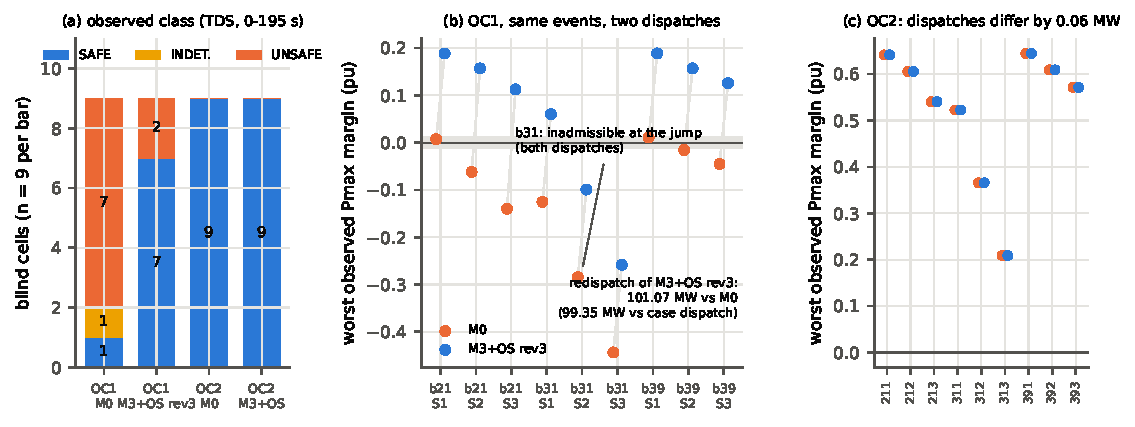
\includegraphics[width=\textwidth]{figures_main/DEC066_F1_M0_vs_M3OS.pdf}
\caption{M0 versus M3+OS (OC1, revision 3) on the same nine blind events. (a) Observed class counts for both operating conditions; (b) worst observed Pmax margin per cell for the two OC1 dispatches (shaded: $\pm U_{D8}$); (c) OC2, where both dispatches differ by 0.06~MW and the outcome is identical (9/9 SAFE), so OC2 does not show an effect of the redispatch. Redispatch of the M3+OS design: 101.07~MW with respect to M0 (99.35~MW with respect to the original case dispatch). ANDES RMS/phasor results.}
\label{fig:f1}
\end{figure*}

\begin{figure*}[t]
\centering
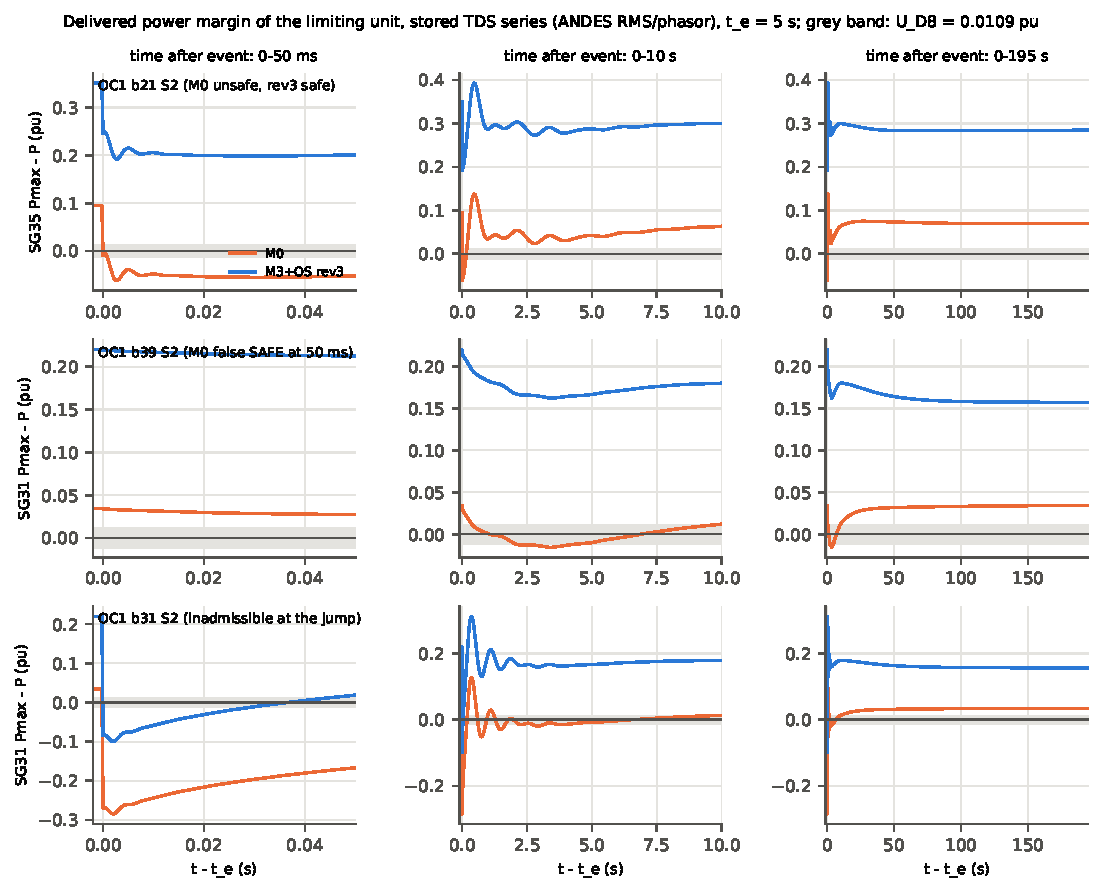
\includegraphics[width=0.85\textwidth]{figures_main/DEC066_F2_critical_transients.pdf}
\caption{Pmax margin of the limiting unit for three OC1 events at the M0 and M3+OS (rev3) dispatches, shown in three time windows after the event ($t_e=5$~s). Top: b21 S2 (violation at M0 within 3~ms, safe at rev3). Middle: b39 S2 (the margin is positive in the first 50~ms at M0 and becomes negative between about 1 and 6~s). Bottom: b31 S2 (inadmissible at the jump for both dispatches).}
\label{fig:f2}
\end{figure*}

\emph{How the redispatch acts.} The M3+OS design moves about 100~MW of generation to the balancing unit SG39 (headroom 529.7 to 429.6~MW) from the units that limit the events: SG31 (headroom 3.4 to 22.0~MW), SG33 (29.3 to 69.3~MW), SG35 (9.5 to 35.1~MW) and GFM36 (14.5 to 30.4~MW) (Fig.~\ref{fig:f6}). The effect is a transfer of pre-event headroom to the critical units, which is what the post-event admissibility condition requires.

\begin{figure}[t]
\centering
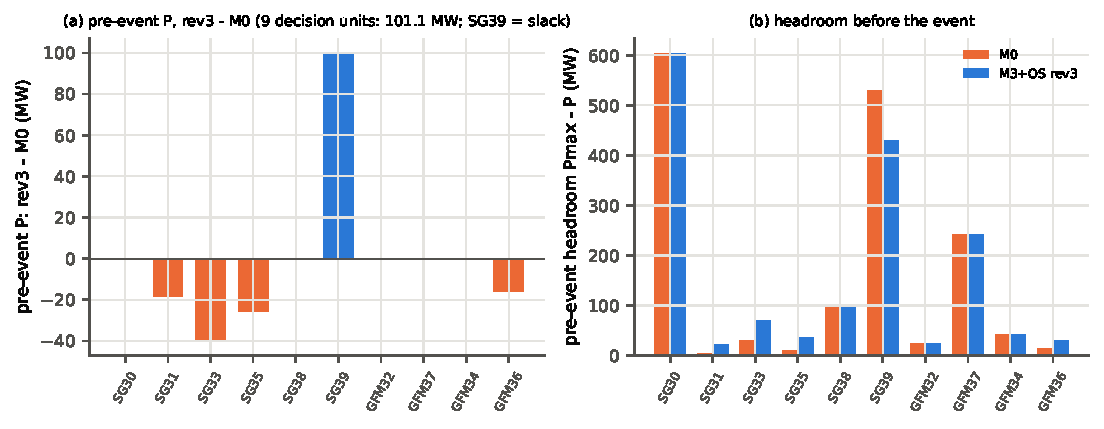
\includegraphics[width=\columnwidth]{figures_main/DEC066_F6_dispatch_by_unit.pdf}
\caption{Pre-event active power change by unit between the M0 and M3+OS (rev3) dispatches (OC1) and headroom to Pmax before the event.}
\label{fig:f6}
\end{figure}

\emph{Comparison with other preventive designs.} In an earlier prospective cohort of 24 simulations (six buses, one amplitude, designs M0, M1 static reserve, M2 jump only, M3 jump plus excursion), M0 violated Pmax in 6 of 6 events, M2 in 1 of 6 (excess 0.0096~pu), and M1 and M3 in none; M3 needed 44.2~MW of redispatch against 156.1~MW for M1 (Table~\ref{tab:dispatches}, Fig.~\ref{fig:f5}a). That cohort used a different design set and a thin margin, and M3+OS was not part of it, so Fig.~\ref{fig:f5} shows two separate datasets and not a single frontier. The cost $J$ and $\sum|\Delta P|$ are effort measures, not prices.

\begin{figure}[t]
\centering
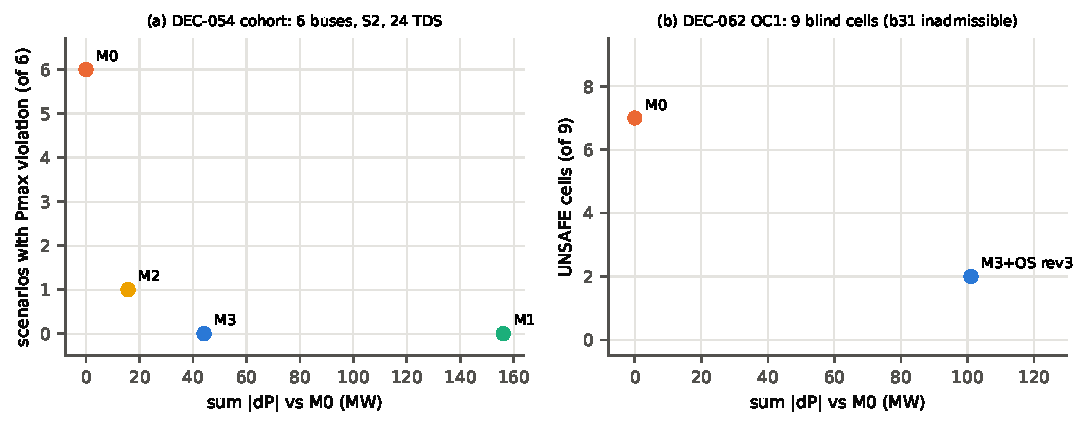
\includegraphics[width=\columnwidth]{figures_main/DEC066_F5_safety_vs_dispatch_effort.pdf}
\caption{Observed Pmax violations against redispatch effort. (a) DEC-054 prospective cohort (24 simulations, S2 at six buses). (b) DEC-062 OC1 blind cells (nine per dispatch).}
\label{fig:f5}
\end{figure}

\subsection{Predictor accuracy and the horizon of the classifier}
\label{sec:predictor}
The design predictor combines the algebraic jump, a dense 0--50~ms evaluation of the post-jump response, and the M3 propagation over 195~s on a grid (2$^{-8}$~s up to 1~s, 0.05~s up to 10~s, 0.5~s afterwards). Over the 36 cells, the predicted 0--50~ms margin has a bias of $+1.7\times10^{-4}$~pu and an RMSE of $4.5\times10^{-4}$~pu with respect to the stored series (Table~\ref{tab:predictor}). Its classification, however, produced the two false SAFE of the study: OC1 M0, b39 S2 and S3, predicted SAFE (50~ms margins 0.027 and 0.024~pu) and observed UNSAFE with worst margins of $-0.0156$ and $-0.0451$~pu at SG31, 3.40 and 3.54~s after the event.

The M3 propagation over 195~s already contains that information, and it was not used by the classifier. Applied to the same cells without re-simulation, it classifies both cells UNSAFE, and 35 of the 36 cells agree with the observed class with no false SAFE; its one disagreement is a false UNSAFE (OC1 M0, b39 S1). Fig.~\ref{fig:f3} shows why the agreement must not be read as accuracy of the worst point: for SG31 the predictor reproduces the observed margin over the first 10~s (the minimum of the observed trajectory at 3--4~s is reproduced within about 0.007~pu), but for SG35 the predicted margin decreases almost linearly after about 20~s, reaching $-0.25$ and $-0.41$~pu at 195~s, while the observed margin remains positive. The overall RMSE at 195~s is therefore 1.92~pu (0.079~pu excluding predictions with margin magnitude of 1~pu or more; 0.011~pu in OC2). A likely cause is that the affine model keeps the post-jump reference rates constant over the whole horizon; this has not been verified in this study. A retrospective sweep of the horizon used for the classification (Table~\ref{tab:horizon}) gives 35/36 agreement with no false SAFE and no false UNSAFE for $T_c=1$, 10 and 60~s, the single disagreement being an INDETERMINATE prediction (never a SAFE one); the choice of $T_c$ was examined on the same cells and is therefore exploratory.

\begin{figure*}[t]
\centering
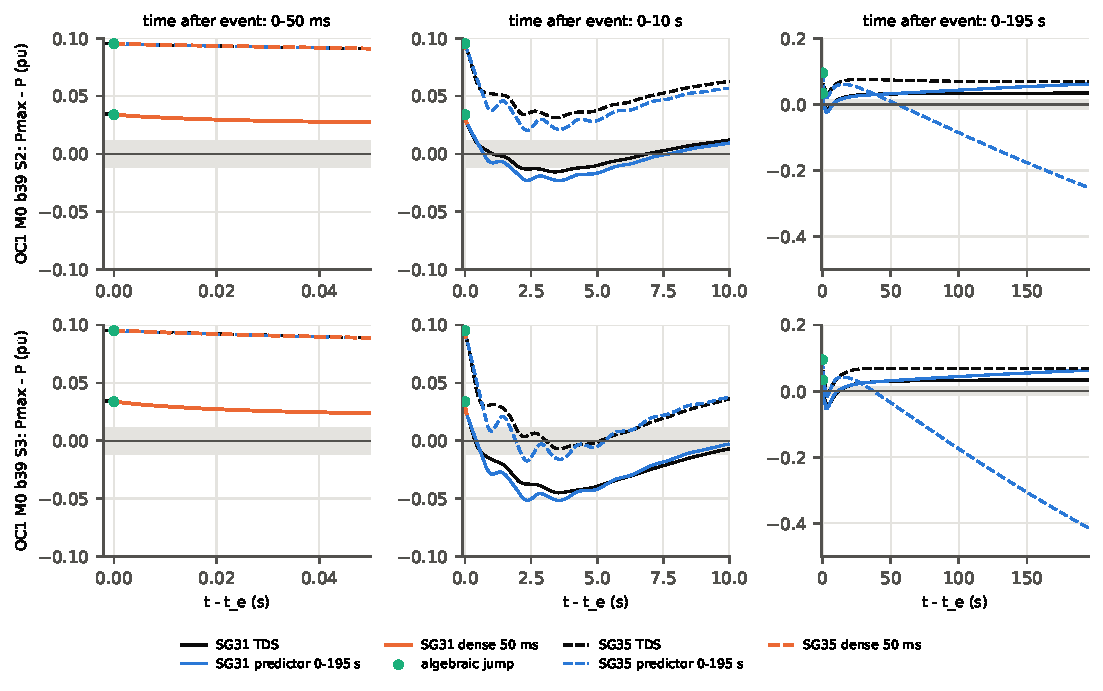
\includegraphics[width=\textwidth]{figures_main/DEC066_F3_predictor_validity.pdf}
\caption{Predictor against time-domain series for the two false-SAFE cells (OC1, M0, bus 39, S2 and S3). Pmax margin of SG31 (solid) and SG35 (dashed): stored ANDES series (black), M3 predictor over 195~s (blue), dense 50~ms predictor (orange) and algebraic jump (green). The 50~ms window ends with positive margin; the violation of SG31 occurs between about 1 and 6~s; the 195~s prediction of SG35 diverges after about 20~s. The same figure at the M3+OS dispatch is in the supplementary file \texttt{DEC066\_F3b}.}
\label{fig:f3}
\end{figure*}

\subsection{Contribution of the overshoot term (ablation)}
\label{sec:ablation}
M3+OS differs from the historical M3 in three changes at once: (i) a dense 0--50~ms evaluation added to the 195~s excursion, (ii) the empirical overshoot term $\varepsilon_{OS}$ ($3.9\times10^{-4}$~pu up, $6.1\times10^{-5}$~pu down, calibrated on 18 design and tuning cells), and (iii) the numerical band $U_{D8}=0.0109$~pu added to both excursion bounds. The third term is 28 times larger than $\varepsilon_{OS}$. The design redispatch rises from 55.3~MW (M3) to 62.1~MW (M3+OS) for the same OC1 design events (Table~\ref{tab:dispatches}). To separate the three components, four additional designs with the same events, objective, solver, seed and starting point are being computed without time-domain simulation: dense only (B), dense plus $\varepsilon_{OS}$ (C), and $U_{D8}$ only (E), compared with M3 (A) and M3+OS (D). \todo{insert ablation table and figure F4 when the designs B, C and E finish; their observed effect requires selected simulations, see below}

\subsection{Limitations}
\label{sec:limitations}
The results come from one network and one plant model in an RMS/phasor simulator, so they say nothing about converter-level or EMT behaviour; Pmax is the operating limit of the case and its temporal tolerance is not known; the disturbances are active-power steps at three evaluation buses, evaluated at two operating conditions, of which only OC1 informs the effect of the dispatch; the 54 evaluation runs were obtained with an access rule modified after tuning and the design revision 3 was made after tuning; the prediction of $Q$, $S$ and voltage is limited to the algebraic jump, and these quantities are only observed in the simulation; the optimisations are local and their solutions are predicted-feasible with large KKT residuals in revision 3 (3.39), so none is presented as optimal; and bus 31 is a counter-example in which the dispatch does not restore admissibility.
